\documentclass{article}
\usepackage{graphicx}
\usepackage{subcaption}
\usepackage[font=small,labelfont=bf]{caption}
\usepackage{array}
\newcolumntype{C}[1]{>{\centering\let\newline\\\arraybackslash\hspace{0pt}}m{#1}}

\begin{document}
	
	\title{Detection of runway closure}
	\maketitle

\section{Objective and method}
We tried to detect the closure of a runway introducing a new variable in our dataset, that indicates the time interval between two consecutive usages of the same runway. To be noticed is the fact that the four runways are indicated with different names, according to the orientation with which they are used. In our analysis we treated as the same runway the couples 26R and 08L (south runway for departures), 26L and 08R (south runway for arrivals), 27R and 09L (north runway for arrivals), 27L and 09R (south runway for departures).
\section{Results}
We show in the figure below the distribution of the time interval between two consecutive flights that use the same runway. In the figure, only intervals of less than one hour are considered, to improve readability.

We can see that the curve is of exponential type, but for the night time it decreases more slowly. This can be explained by the fact that there are less movements at night, and for this reason the time interval between two consecutive movements is longer.

\begin{figure}[h]
	\centering
	\begin{subfigure}[b]{.49\textwidth}
		\centering
		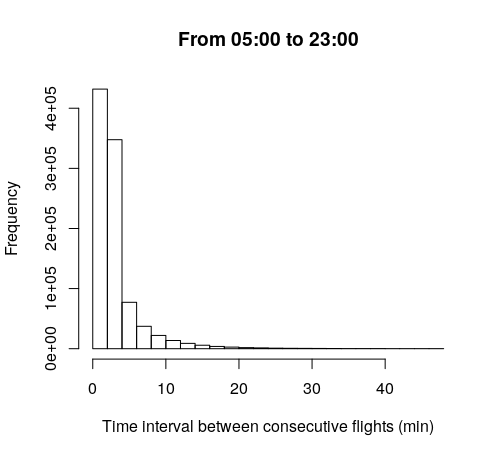
\includegraphics[width=5.8cm]{day.png}
		\label{day}
	\end{subfigure}%
	\begin{subfigure}[b]{.49\textwidth}
		\centering
		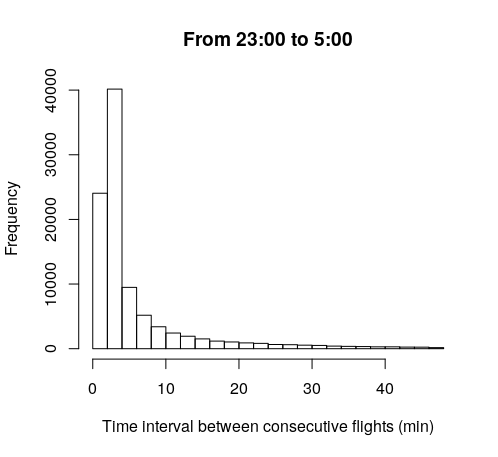
\includegraphics[width=5.8cm]{night.png}
		
		\label{night}
	\end{subfigure}
\end{figure}

From the table below, we can notice that every day at least one of the four runways were closed for at least one hour, and in the 98\% of the days analyzed at least one runway have been closed for at least four hours, and within those days the majority closures happened from 11 p.m. to 5 a.m..
We see that for 4 times a runway were closed for more than one day. Looking at those data, what emerges is that the southern runway for departures were closed for 4 days from 14/11/19 to 18/11/19, while the southern runway for arrivals were closed for three months, from 07/07/18 to 09/10/18, with an interruption in the closure where a few aircrafts use the runway on 01/08/18 and 05/09/18.

\begin{table}[h!!!!!!!!!!!!!!!]
\begin{tabular}{C{2cm}|C{2.5cm}|C{2.5cm}|C{2.5cm}}
	\textbf{Time interval (hours)} & \textbf{N of days of closure}& \textbf{N of days of night time closure} & \textbf{N of days of day time closure}\\
	\hline
	1 & 790 (100\%) & 789 (99\%)& 227 (35\%)\\
	2 & 789 (99\%)& 786 (99\%)& 112 (14\%)\\
	3 & 786 (99\%)& 783 (99\%)& 83 (10\%)\\
	4 & 777 (98\%)& 774 (97\%)& 65 (8\%)\\
	5 & 615 (77\%)& 591 (77\%)& 56 (7\%)\\
	6 & 221 (27\%)& 174 (26\%)& 52 (6\%)\\
	7 & 32 (4\%)& 17 (3\%)& 15 (1\%)\\
	24 & 4 (0,5\%)& 2(0,2\%) &2 (0,2\%) \\
\end{tabular}
\caption{Table of the occurrences of days in which a closure that lasted more than the time interval indicated in the first column happened. The third column indicates the number of days where the closure occured between 11 p.m. and 5 a.m., the fourth column between 5 a.m. and 11 p.m.. The total number of days analyzed were 790.}
\end{table}


The distribution of closures within the four runways is quite uniform, as it is shown in the table below.	

\begin{table}[h!!!!!!!!!!!!!!!]
	\begin{tabular}{C{3cm}|C{2cm}|C{2cm}|C{2cm}|C{2cm}}
		                            &
		\textbf{North for Arrivals} & \textbf{North for Departures}& \textbf{South for Arrivals} & \textbf{South for Departures}\\
		\hline
		 Night time closure& 373 & 350 & 364 & 376\\
		 Day time closure& 16 & 25 & 13 & 26\\
	\end{tabular}
	\caption{Number of days where a closure of more than 4 hours occurred, devided by runway. We consider night time the interval between 11 p.m. and 5 p.m.}
\end{table}

We show below the number of closures (and not only of days of closure) of more than one hour and of more than four hours as a function of the hour for the whole data set.

We can notice that closures of more than 4 hours occur quite only at night, while closures of more than one hour occur more frequently also around 2 p.m., when there is more ground traffic. We expect the closures of 2 p.m. to have a big impact on ground traffic.

	\begin{figure}[h]
	\centering
		\begin{subfigure}[b]{.49\textwidth}
		\centering
		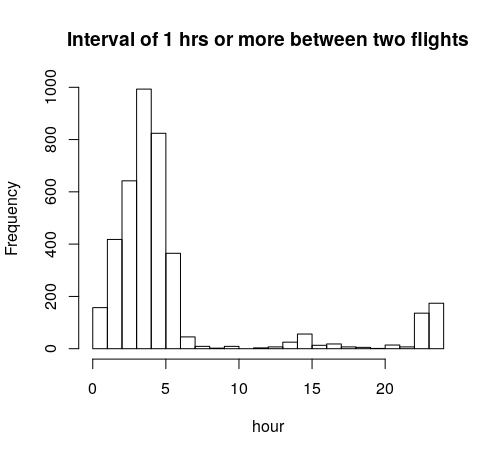
\includegraphics[width=6cm]{interval1hr.png}
		\label{1hr}
		\end{subfigure}%
		\begin{subfigure}[b]{.49\textwidth}
		\centering
		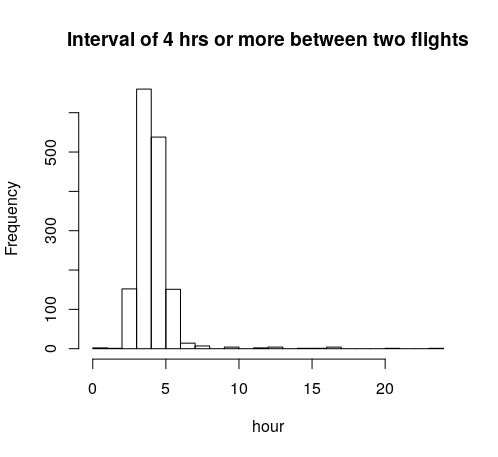
\includegraphics[width=6cm]{interval4hr.png}
		\label{4hr}
	\end{subfigure}
\caption{Histogram of the hours at which closures of more than 1 hour (left side) or more than 4 hours (right side) occur.}
	\end{figure}


\end{document}